% !TEX root = paper.tex
\iflong
\else
\vspace{-2mm}
\fi
\section{Preferred replacement path passes through $t_s$}
\label{sec:passes}
\iflong
Under this assumption, we only need to find the preferred replacement path from $s$ to $t_s$ avoiding $e$. Note that we already know $|t_st|$ length via $B_0(t_{s},t)$. We use the following additional data structures:



\begin{itemize}[leftmargin=*,noitemsep,nolistsep]
\item $B_2$: For $x \in S \cup \TT$ and $y \in V$, $B_2(x,y)$ contains the vertex $w$ on $xy$ path such that $|yw| = 2^{\lfloor \log |xy| \rfloor}$, or in words, the vertex nearest to $x$ whose distance from $y$ is a power of 2. The size of $B_2$ is $\tilde O((\sigma+\sqrt{n\sigma})n) = \tilde O(\sigma^{1/2}n^{3/2})$.

\item $B_3$: For $x \in V$ and $y \in \TT$, $B_4(x,y, \oplus2^i)$
contains the shortest path from $x$ to $y$ avoiding every
$2^i$-th
edge on the path $xy$ from $x$ (where $i \le \log \lfloor
|xy| \rfloor$). Since $|\TT| = \tilde O(\sqrt{n \sigma})$, the size
of $B_3$ is $\tilde O( \sigma^{1/2} n^{3/2} )$.

\item $B_4$: For $s \in S$ and $x \in V$, $B_4(s,x, \ominus2^i)$ contains  the shortest path from $s$ to $x$ avoiding the $2^i$-th
edge on the path $sx$ from $x$ (where $i \le \log \lfloor |sx| \rfloor$). The size of $B_4$ is $ \tilde O( n \sigma) = \tilde O( \sigma^{1/2} n^{3/2} )$.



\item $B_5$: For every $s \in S$ and $x \in \TT$, $B_5(s,x, [\oplus 2^i, \ominus 2^j])$ contains the shortest path from $s$ to $x$ avoiding the sub path
that start from $2^i$-th vertex from $s$ and ends at $2^j$-th
vertex from $x$ on the path $sx$ (where  $i,j \le \log \lfloor sx \rfloor$). The size of $B_5$ is $\tilde O(\sigma^{3/2} n^{1/2}) = \tilde O( \sigma^{1/2} n^{3/2} )$.


\end{itemize}

\begin{figure}
\centering

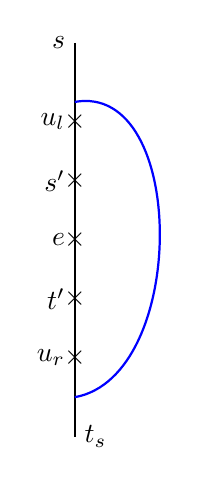
\begin{tikzpicture}[scale=1]

\coordinate (x) at (0,5);
\coordinate (y) at (0,0);
\coordinate (u) at (0,2.5);
\coordinate (ul) at (0,1);
\coordinate (ur) at (0,4);

\coordinate (x1) at (0,1.75);
\coordinate (y1) at (0,3.25);

\draw[thick](x)--(y);
\node[left] at (x){$s$};
\node[right] at (y){$t_{s}$};

\node[left] at (u){$e$};
\node at (u){$\times$};
\node[left] at (ul){$u_r$};
\node at (ul){$\times$};
\node[left] at (ur){$u_l$};
\node at (ur){$\times$};

\node[left] at (x1){$t'$};
\node at (x1){$\times$};
\node[left] at (y1){$s'$};
\node at (y1){$\times$};

\draw[thick,blue] (0,0.5) to[out=10,in=10] node[pos=0.2,
left]
{ } (0,4.25);
\end{tikzpicture}
\caption{The hardest part of the distance oracle, when the
replacement path neither passes through $u_l$ not $u_r$.}
\end{figure}

\noindent   Assume that we get a query
{\sc Q}($s,t,e(u,v)$), that is, find the shortest path from
$s$ to $t$ avoiding $e$. Assume without loss of generality that $u$ is closer to $s$ on $st$ path than $v$. We answer this query as follows:
first we find the distance of $v$ from $s$, via $B_0(s,v)$. If $B_0(s,v)$ is a power of 2 then
we can directly use $B_3(s,t_s, \oplus |sv|) + B_0(t_s,t)$. Else, let $u_l \leftarrow  B_2(s,v)$ and
$u_r \leftarrow B_2(t_s,u)$. Here $u_l$ is the nearest vertex to $s$ on $vs$ path whose
 distance from $v$ is a power of 2. Similarly, $u_r$ is the nearest vertex to $t_s$ on $ut_s$ path whose distance form $u$ is a power of 2.    There are three cases now:

\begin{enumerate}[noitemsep,nolistsep]
\item  The  preferred replacement path passes through $u_l$.

\item  The preferred replacement path passes through $u_r$.

\item The preferred replacement path neither passes through $u_l$
nor $u_r$.

\end{enumerate}
\noindent For the first case, we  can report $B_0(s,u_l) + B_3(u_l, t_{s}, \oplus|u_lv|) + B_0(t_s,t) $. For the second case, we can report $B_4(s,u_r, \ominus  |uu_r|) + B_0(u_r,t_s) + B_0(t_s,t)$ . The hardest
case is when the preferred replacement path neither passes through
$u_l$ nor $u_r$. Let $s'$ be the farthest
vertex  on $sv$ path from $s$ whose distance is a power
of 2, that is $|ss'| = 2^{\lfloor \log |sv| \rfloor}$. Similarly let $t'$ be the farthest vertex on $t_{s}u$
path from $t_s$ whose distance is a power
of 2. Now,
we can  report the shortest path from $s$ to $t_{s}$ avoiding
$[s',t']$ -- this is also stored in $B_5(s,t_s,[\oplus 2^{\lfloor \log |sv| \rfloor}, \ominus 2^{\lfloor
\log |t_su| \rfloor}] )$. By construction, if the shortest path avoids $[u_l,u_r]$, then it also
avoids $[s',t']$. Thus we can return $B_5(s,t_s,[\oplus 2^{\lfloor \log |sv| \rfloor}, \ominus 2^{\lfloor
\log |t_su| \rfloor}] ) +\ B_0(t_s,t)$ as the length  of the preferred replacement path.
The reader can check that the running time of our algorithm
is $O(1)$ as we have to check $B_0,B_1,B_2,B_3,B_4,B_5$ constant number of times.
For the correctness of the above procedure, please refer to \cite{DemetrescuTCR08,DuanP09}.
\else
Since this case is a generalization of the techniques developed by
Demetrescu et. al. \cite{DemetrescuTCR08}, concerned reader may read
the full version of the paper for details -- where we show that there exists a data-structure
of size $\tilde O(\sigma^{1/2}n^{3/2})$ which takes $O(1)$ time to find a replacement
path from $s$ to $t$ that avoids $e$ but passes through $t_s$.
\fi

Now, we move on to the harder case, that is, replacement paths avoid $t_s$ too. For this, we will  fix a vertex $t$. We will show
that the query
${\sc Q}(s,t,e(u,v))$  can be answered
in $\tilde O(1)$ using $\tilde O(\sqrt{\sigma n})$ space.
This immediately implies that we can answer exact queries
in $\tilde O(1)$ time using $\tilde O(\sigma^{1/2} n^{3/2})$
space.

%In the rest of the paper, we try to find a distance
%oracle for a fixed $t$.
